\documentclass[14pt, a4paper]{article}
\usepackage[14pt]{extsizes} % для того чтобы задать нестандартный 14-ый размер шрифта
\usepackage[utf8]{inputenc}
\usepackage{cmap}
\usepackage{multirow}

\usepackage{titlesec}
\usepackage{enumitem}
\setlist{nolistsep, itemsep=0.3cm,parsep=0pt,leftmargin=1.5cm}

\titleformat*{\section}{\filcenter\bfseries\MakeUppercase}
\titleformat*{\subsection}{\bfseries\filcenter\MakeUppercase}
\titleformat*{\subsubsection}{\bfseries\filcenter\MakeUppercase}
\titleformat*{\paragraph}{\bfseries\filcenter\MakeUppercase}
\titleformat*{\subparagraph}{\bfseries\filcenter\MakeUppercase}


\makeatletter
\renewcommand{\l@section}{\@dottedtocline{1}{0em}{1.25em}}
\renewcommand{\l@subsection}{\@dottedtocline{2}{1.25em}{1.75em}}
\renewcommand{\l@subsubsection}{\@dottedtocline{3}{2.75em}{2.6em}}
\makeatother

\usepackage{graphicx}
\usepackage{natbib}
\usepackage{caption} 
\usepackage[russian]{babel}
\usepackage{setspace,amsmath}
\usepackage[left=30mm, top=15mm, right=10mm, bottom=20mm, nohead, footskip=10mm]{geometry} % настройки полей документа
\usepackage{indentfirst} % отделять первую строку раздела абзацным отступом тоже  

\linespread{1.5} % полуторный интервал
\usepackage{fontspec}
\setmainfont{Times New Roman}
\usepackage{caption}
\captionsetup[table]{singlelinecheck=false,justification=raggedright}

\usepackage{pgfplots}
\pgfplotsset{compat=1.9}
\begin{document}

Последовательность для тестирования алгоритма квантования весов была составлена из первых 70 кадров Woman. Алгоритм DLT на данной последовательности без квантования весов работал в течение 47.51 секунд и с $fps = 1.47$ кадров в секунду.

\section*{Зависимость времени работы программы слежения от числа уровней квантования}

\begin{table}[h!]
\caption*{Таблица 2.2 -- Зависимость времени от числа уровней квантования}
\begin{tabular}{|c|c|c|c|}
\hline
L   & \begin{tabular}[c]{@{}c@{}}Время работы\\  программы\end{tabular} & \begin{tabular}[c]{@{}c@{}}Количество кадров\\  в секунду (fps)\end{tabular} & \begin{tabular}[c]{@{}c@{}}Время квантования\\   матриц\end{tabular} \\ \hline
2   & 75.4                                                              & 0.93                                                                         & 10.2                                                                 \\ \hline
4   & 73.8                                                              & 0.95                                                                         & 10.1                                                                 \\ \hline
8   & 74.6                                                              & 0.94                                                                         & 12.3                                                                 \\ \hline
16  & 72.6                                                              & 0.96                                                                         & 18.6                                                                 \\ \hline
32  & 72.6                                                              & 0.96                                                                         & 30.1                                                                 \\ \hline
64  & 74.6                                                              & 0.94                                                                         & 54                                                                   \\ \hline
128 & 45.7                                                              & 1.53                                                                         & 105.3                                                                \\ \hline
256 & 43.9                                                              & 1.6                                                                          & 202                                                                  \\ \hline                     
\end{tabular}
\end{table}

\begin{figure}[h!]
    \centering
    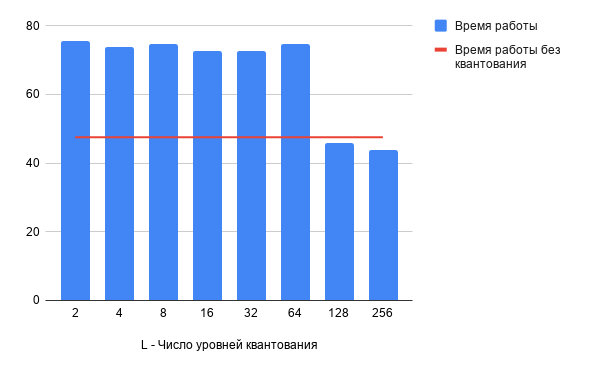
\includegraphics[width = 14cm]{tests/img/time.png}
    \caption*{Рисунок 1 -- Зависимость времени от числа уровней квантования}
\end{figure}

\section*{Зависимость среднего смещения центра рамки захвата (в пикселах) от числа уровней квантования}

\begin{table}[h!]
\caption*{Таблица 2.3 -- Зависимость смещения центра от числа уровней квантования}
\begin{tabular}{|c|c|c|}
\hline
\multirow{2}{*}{L} & \multicolumn{2}{c|}{\begin{tabular}[c]{@{}c@{}}Среднее смещение\end{tabular}}                                                                      \\ \cline{2-3} 
                   & \begin{tabular}[c]{@{}c@{}}по горизонтали (по координате x)\end{tabular} & \begin{tabular}[c]{@{}c@{}}по вертикали (по координате y)\end{tabular} \\ \hline
2                             & 16,2                                   & 41,9                                 \\ \hline
4                             & 24,4                                   & 30,2                                 \\ \hline
8                             & 41                                     & 7,6                                  \\ \hline
16                            & 8,4                                    & 17                                   \\ \hline
32                            & 11,8                                   & 13                                   \\ \hline
64                            & 7,2                                    & 44,7                                 \\ \hline
128                           & 1,6                                    & 1,6                                  \\ \hline
256                           & 0,5                                    & 0,9                                  \\ \hline
\end{tabular}
\end{table}

\begin{figure}[h!]
    \centering
    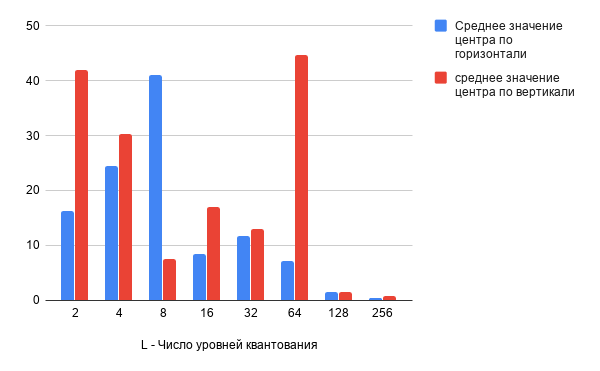
\includegraphics[width = 14 cm]{tests/img/sm.png}
    \caption*{Рисунок 2 -- Зависимость смещения центра от числа уровней квантования}
\end{figure}

\newpage

\section*{Смещение центра рамки в зависимости от номера кадра}

 \begin{figure}[h!]
    \centering
    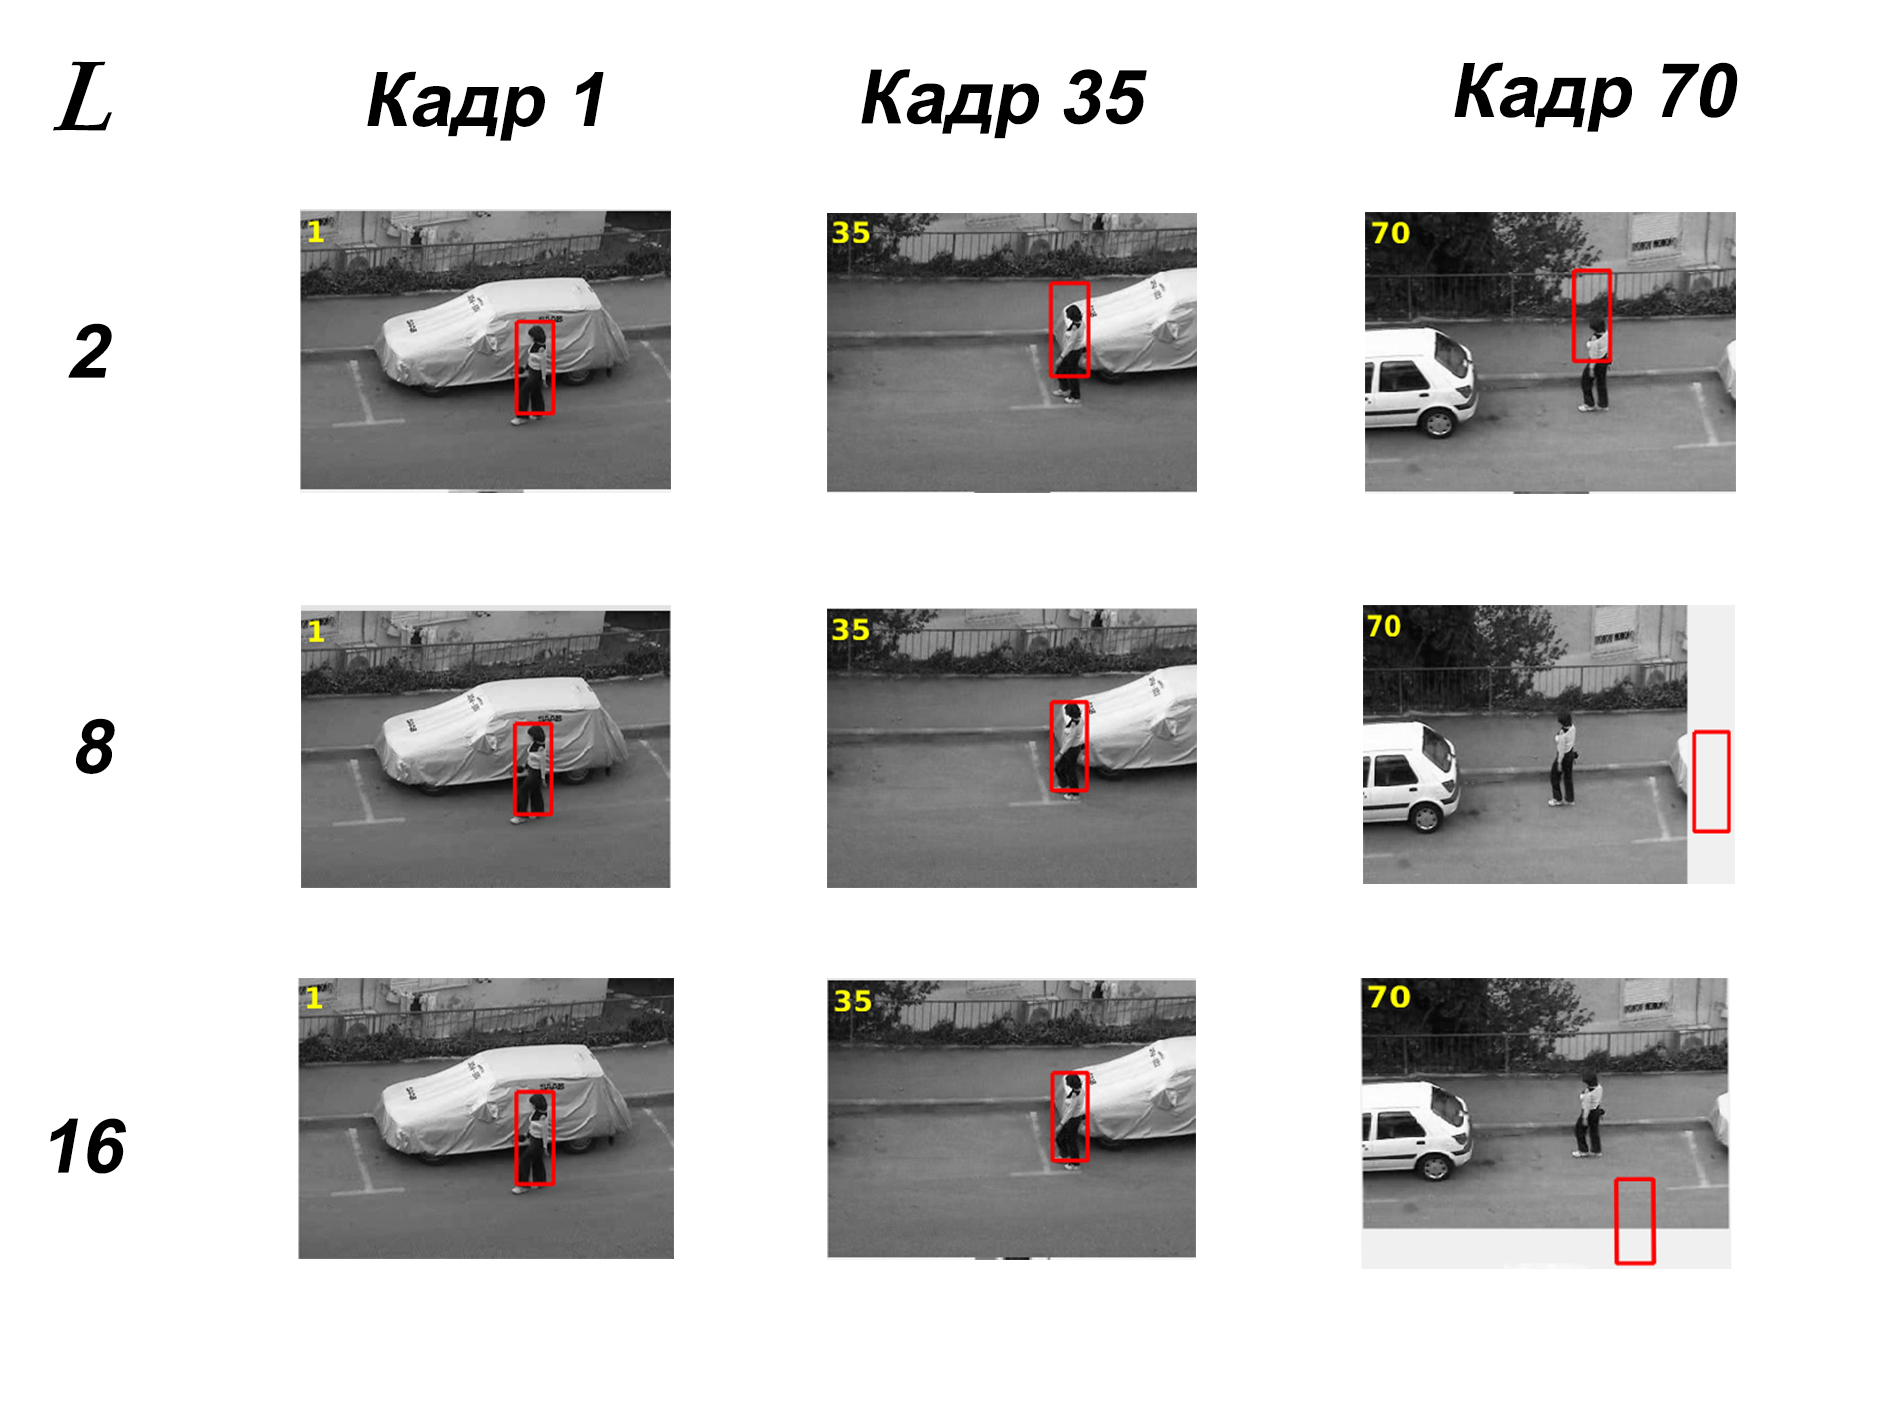
\includegraphics[width=11cm]{tests/img/Bez_imeni-1.jpg}
    \caption*{Рисунок 3 - Смещение рамки при $L = 2,8,32$}
\end{figure}

 \begin{figure}[h!]
    \centering
    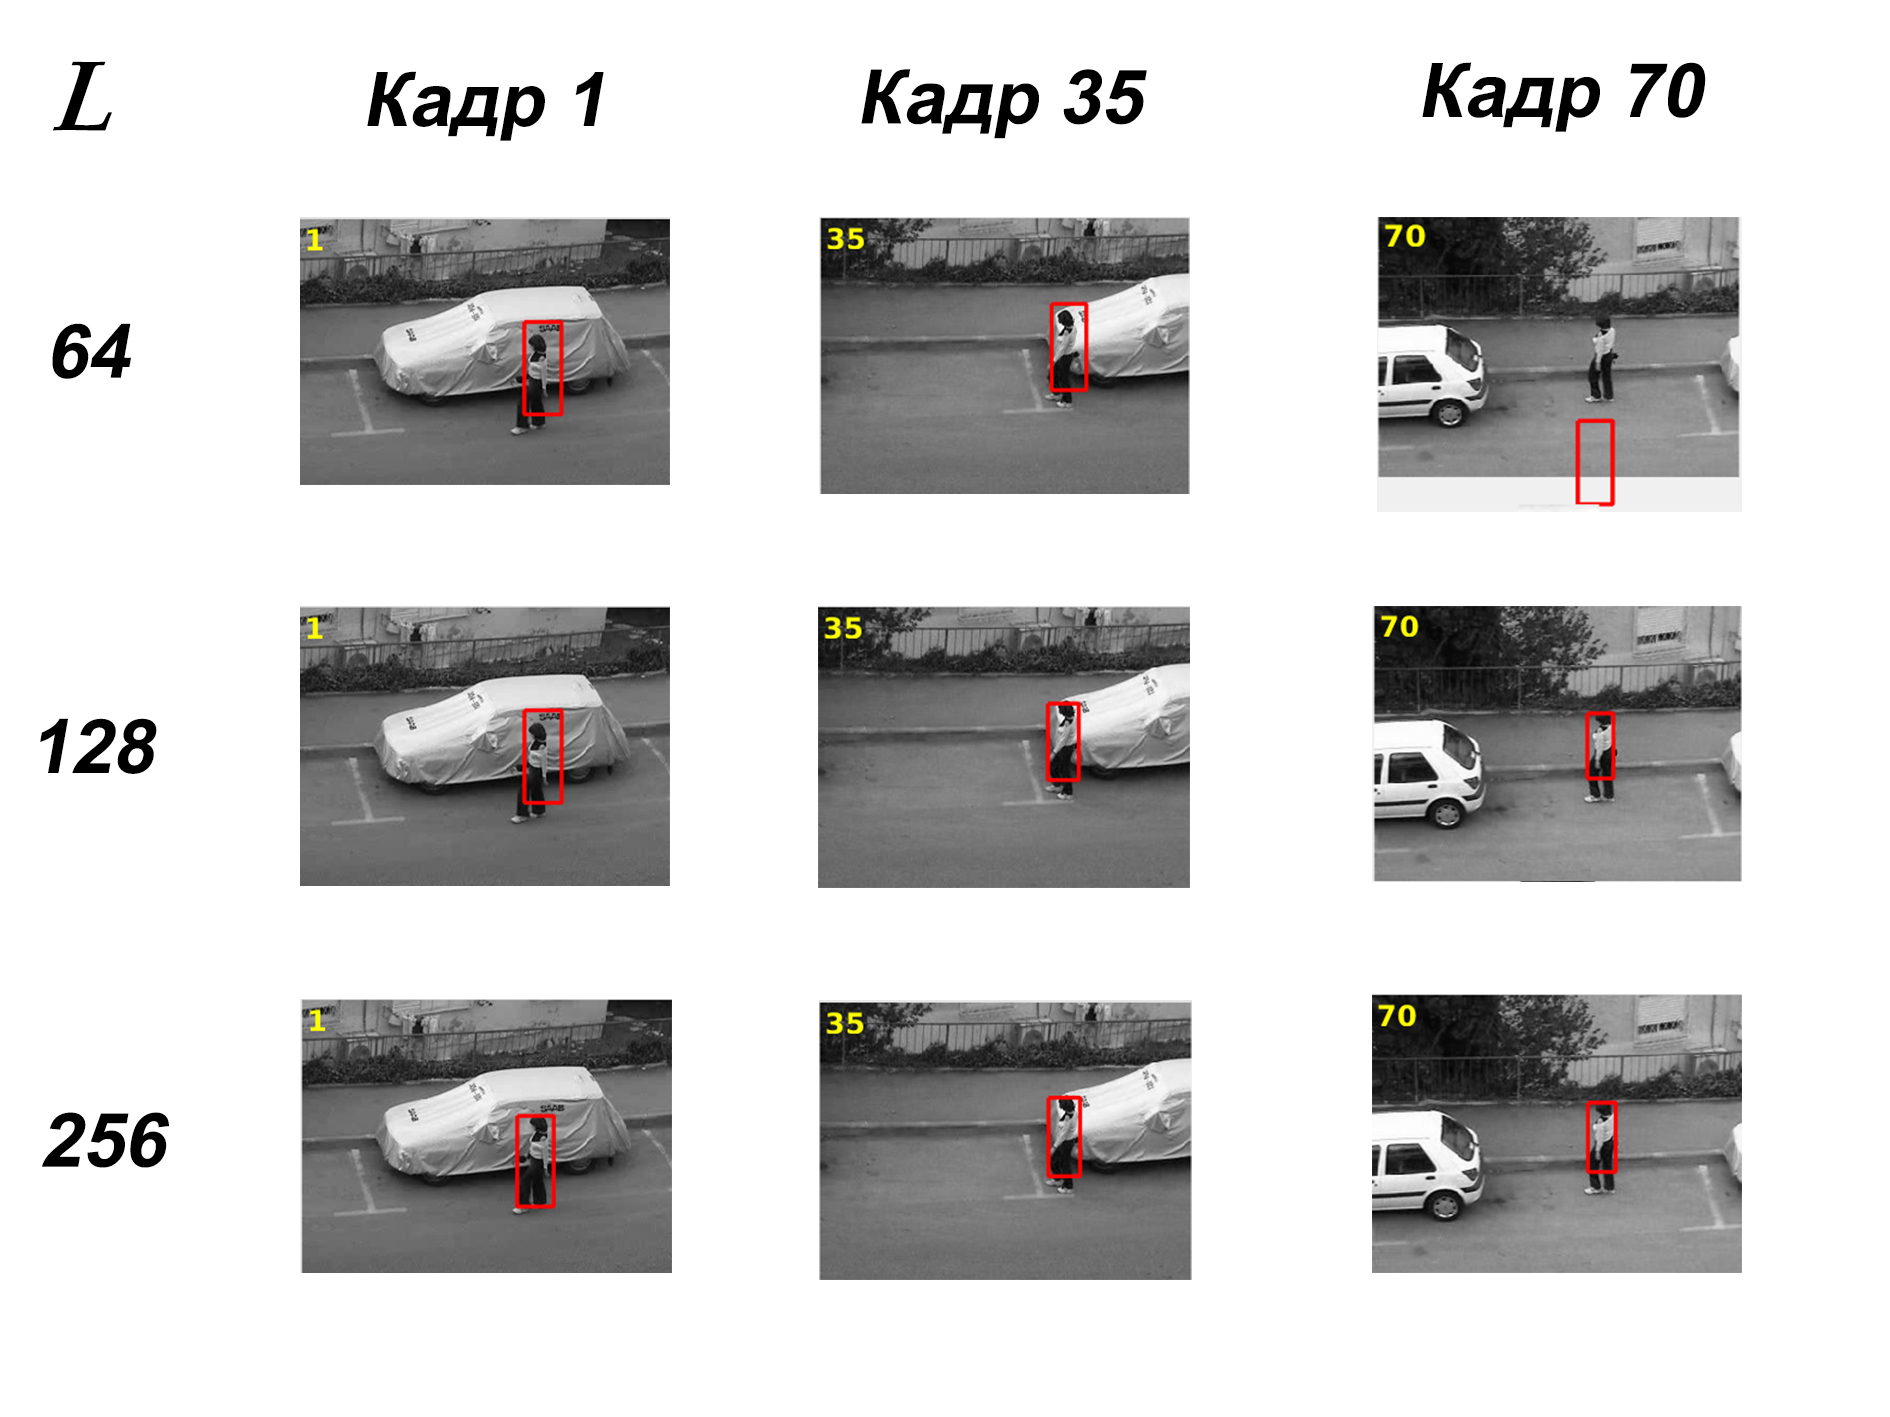
\includegraphics[width=11cm]{tests/img/Bez_imeni-2.jpg}
    \caption*{Рисунок 4 - Смещение рамки при $L = 128,512,1024$}
\end{figure}

\begin{table}[h!]
\caption*{Таблица 1 -- Смещение центра по горизонтали. Кадры 1-29}
\begin{tabular}{|c|c|c|c|c|c|c|c|c|}
\hline
Номер кадра: & L=2   & L=4   & L=8   & L=16  & L=32  & L=64 & L=128 & L=256 \\ \hline
1            & 1.1   & 1.1   & 0     & 0     & 0     & 7.7  & 7.7   & 0     \\ \hline
2            & 0     & 0     & 0     & 0     & 16.5  & 1.1  & 1.1   & 0     \\ \hline
3            & 2.2   & 6.6   & 1.1   & 1.1   & 2.2   & 1.1  & 4.4   & 0     \\ \hline
4            & 4.4   & 19.8  & 1.1   & 2.2   & 5.5   & 3.3  & 7.7   & 1.1   \\ \hline
5            & 11    & 3.3   & 0     & 0     & 6.6   & 4.4  & 5.5   & 1.1   \\ \hline
6            & 7.7   & 15.4  & 1.1   & 1.1   & 1.1   & 4.4  & 1.1   & 0     \\ \hline
7            & 4.4   & 4.4   & 1.1   & 1.1   & 0     & 2.2  & 1.1   & 0     \\ \hline
8            & 34.1  & 16.5  & 1.1   & 0     & 4.4   & 4.4  & 1.1   & 0     \\ \hline
9            & 3.3   & 3.3   & 1.1   & 1.1   & 4.4   & 5.5  & 1.1   & 1.1   \\ \hline
10           & 18.7  & 2.2   & 1.1   & 1.1   & 9.9   & 8.8  & 0     & 0     \\ \hline
11           & 11    & 6.6   & 0     & 0     & 7.7   & 8.8  & 0     & 1.1   \\ \hline
12           & 23.1  & 3.3   & 1.1   & 1.1   & 3.3   & 6.6  & 0     & 0     \\ \hline
13           & 9.9   & 23.1  & 0     & 0     & 1.1   & 5.5  & 2.2   & 0     \\ \hline
14           & 28.6  & 9.9   & 0     & 0     & 0     & 7.7  & 2.2   & 0     \\ \hline
15           & 52.8  & 6.6   & 1.1   & 1.1   & 5.5   & 6.6  & 3.3   & 0     \\ \hline
16           & 6.6   & 9.9   & 1.1   & 1.1   & 7.7   & 7.7  & 1.1   & 0     \\ \hline
17           & 18.7  & 9.9   & 1.1   & 1.1   & 1.1   & 4.4  & 2.2   & 1.1   \\ \hline
18           & 5.5   & 35.2  & 0     & 0     & 1.1   & 4.4  & 1.1   & 0     \\ \hline
19           & 4.4   & 16.5  & 1.1   & 1.1   & 2.2   & 4.4  & 1.1   & 0     \\ \hline
20           & 2.2   & 4.4   & 1.1   & 1.1   & 0     & 6.6  & 1.1   & 0     \\ \hline
21           & 4.4   & 6.6   & 0     & 0     & 1.1   & 5.5  & 1.1   & 0     \\ \hline
22           & 11    & 18.7  & 0     & 0     & 1.1   & 7.7  & 1.1   & 1.1   \\ \hline
23           & 9.9   & 41.8  & 0     & 0     & 2.2   & 5.5  & 1.1   & 0     \\ \hline
24           & 3.3   & 1.1   & 0     & 0     & 1.1   & 6.6  & 1.1   & 0     \\ \hline
25           & 35.2  & 63.8  & 1.1   & 1.1   & 1.1   & 6.6  & 1.1   & 0     \\ \hline
26           & 4.4   & 14.3  & 1.1   & 1.1   & 1.1   & 3.3  & 1.1   & 0     \\ \hline
27           & 1.1   & 2.2   & 1.1   & 0     & 4.4   & 6.6  & 2.2   & 0     \\ \hline
28           & 11    & 25.3  & 1.1   & 0     & 2.2   & 4.4  & 1.1   & 0     \\ \hline
29           & 6.6   & 20.9  & 0     & 0     & 1.1   & 6.6  & 1.1   & 1.1   \\ \hline
30           & 1.1   & 25.3  & 1.1   & 1.1   & 1.1   & 4.4  & 1.1   & 0     \\ \hline
31           & 1.1   & 52.8  & 1.1   & 1.1   & 1.1   & 4.4  & 1.1   & 1.1   \\ \hline
\end{tabular}
\end{table}



\begin{table}[h!]
\caption*{Таблица 2 -- Смещение центра по горизонтали. Кадры 30-70}
\begin{tabular}{|c|c|c|c|c|c|c|c|c|}
\hline
Номер кадра: & L=2   & L=4   & L=8   & L=16  & L=32  & L=64 & L=128 & L=256 \\ \hline
32           & 5.5   & 48.4  & 1.1   & 1.1   & 1.1   & 5.5  & 1.1   & 0     \\ \hline
33           & 3.3   & 19.8  & 2.2   & 2.2   & 5.5   & 4.4  & 1.1   & 1.1   \\ \hline
34           & 19.8  & 16.5  & 0     & 0     & 1.1   & 6.6  & 1.1   & 0     \\ \hline
35           & 2.2   & 19.8  & 2.2   & 2.2   & 4.4   & 4.4  & 1.1   & 1.1   \\ \hline
36           & 7.7   & 42.9  & 1.1   & 1.1   & 1.1   & 5.5  & 1.1   & 0     \\ \hline
37           & 0     & 45.1  & 1.1   & 1.1   & 1.1   & 4.4  & 1.1   & 0     \\ \hline
38           & 11    & 2.2   & 2.2   & 2.2   & 1.1   & 1.1  & 2.2   & 1.1   \\ \hline
39           & 9.9   & 12.1  & 4.4   & 4.4   & 3.3   & 0    & 3.3   & 1.1   \\ \hline
40           & 6.6   & 24.2  & 2.2   & 1.1   & 3.3   & 3.3  & 1.1   & 0     \\ \hline
41           & 7.7   & 7.7   & 2.2   & 2.2   & 2.2   & 23.1 & 1.1   & 1.1   \\ \hline
42           & 3.3   & 31.9  & 0     & 2.2   & 1.1   & 4.4  & 0     & 0     \\ \hline
43           & 34.1  & 29.7  & 1.1   & 1.1   & 2.2   & 5.5  & 0     & 0     \\ \hline
44           & 9.9   & 15.4  & 0     & 3.3   & 129.8 & 18.7 & 2.2   & 1.1   \\ \hline
45           & 40.7  & 23.1  & 118.8 & 126.5 & 135.3 & 13.2 & 0     & 0     \\ \hline
46           & 46.2  & 45.1  & 122.1 & 1.1   & 2.2   & 3.3  & 1.1   & 1.1   \\ \hline
47           & 11    & 67.1  & 125.4 & 1.1   & 0     & 3.3  & 0     & 0     \\ \hline
48           & 17.6  & 28.6  & 2.2   & 1.1   & 0     & 2.2  & 3.3   & 1.1   \\ \hline
49           & 19.8  & 37.4  & 122.1 & 1.1   & 1.1   & 1.1  & 3.3   & 2.2   \\ \hline
50           & 74.8  & 16.5  & 133.1 & 2.2   & 1.1   & 27.5 & 4.4   & 2.2   \\ \hline
51           & 60.5  & 9.9   & 132   & 2.2   & 4.4   & 18.7 & 4.4   & 3.3   \\ \hline
52           & 66    & 26.4  & 133.1 & 2.2   & 2.2   & 25.3 & 4.4   & 2.2   \\ \hline
53           & 6.6   & 2.2   & 1.1   & 1.1   & 140.8 & 1.1  & 2.2   & 1.1   \\ \hline
54           & 33    & 102.3 & 1.1   & 1.1   & 5.5   & 4.4  & 1.1   & 0     \\ \hline
55           & 2.2   & 49.5  & 1.1   & 1.1   & 46.2  & 16.5 & 1.1   & 0     \\ \hline
56           & 14.3  & 14.3  & 1.1   & 35.2  & 38.5  & 19.8 & 2.2   & 2.2   \\ \hline
57           & 13.2  & 20.9  & 0     & 61.6  & 53.9  & 8.8  & 1.1   & 0     \\ \hline
58           & 3.3   & 2.2   & 146.3 & 4.4   & 56.1  & 9.9  & 0     & 0     \\ \hline
59           & 12.1  & 11    & 149.6 & 0     & 63.8  & 8.8  & 0     & 0     \\ \hline
60           & 2.2   & 7.7   & 151.8 & 1.1   & 1.1   & 7.7  & 0     & 0     \\ \hline
61           & 101.2 & 6.6   & 149.6 & 1.1   & 2.2   & 1.1  & 0     & 0     \\ \hline
62           & 7.7   & 3.3   & 143   & 39.6  & 1.1   & 13.2 & 1.1   & 1.1   \\ \hline
63           & 20.9  & 101.2 & 143   & 1.1   & 2.2   & 7.7  & 1.1   & 1.1   \\ \hline
64           & 18.7  & 17.6  & 146.3 & 47.3  & 0     & 9.9  & 0     & 0     \\ \hline
65           & 25.3  & 23.1  & 155.1 & 0     & 3.3   & 3.3  & 0     & 0     \\ \hline
66           & 50.6  & 77    & 145.2 & 1.1   & 2.2   & 2.2  & 1.1   & 0     \\ \hline
67           & 6.6   & 56.1  & 146.3 & 56.1  & 2.2   & 8.8  & 1.1   & 0     \\ \hline
68           & 6.6   & 61.6  & 141.9 & 58.3  & 5.5   & 13.2 & 1.1   & 1.1   \\ \hline
69           & 12.1  & 67.1  & 159.5 & 53.9  & 1.1   & 13.2 & 0     & 0     \\ \hline
70           & 4.4   & 44    & 159.5 & 42.9  & 1.1   & 6.6  & 1.1   & 0     \\ \hline
\end{tabular}
\end{table}


\begin{table}[h!]
\caption*{Таблица 3 -- Смещение центра по вертикали. Кадры 1-29}
\begin{tabular}{|c|c|c|c|c|c|c|c|c|}
\hline
Номер кадра: & L=2   & L=4  & L=8  & L=16  & L=32  & L=64  & L=128 & L=256 \\ \hline
1            & 4.8   & 4.8  & 2.4  & 2.4   & 3.6   & 14.4  & 14.4  & 0     \\ \hline
2            & 9.6   & 9.6  & 1.2  & 1.2   & 14.4  & 18    & 1.2   & 1.2   \\ \hline
3            & 2.4   & 25.2 & 0    & 0     & 3.6   & 16.8  & 1.2   & 0     \\ \hline
4            & 3.6   & 9.6  & 0    & 0     & 3.6   & 15.6  & 1.2   & 0     \\ \hline
5            & 7.2   & 32.4 & 1.2  & 1.2   & 4.8   & 18    & 1.2   & 1.2   \\ \hline
6            & 10.8  & 9.6  & 1.2  & 1.2   & 2.4   & 18    & 2.4   & 1.2   \\ \hline
7            & 13.2  & 1.2  & 0    & 0     & 2.4   & 18    & 1.2   & 0     \\ \hline
8            & 21.6  & 28.8 & 1.2  & 0     & 4.8   & 13.2  & 3.6   & 1.2   \\ \hline
9            & 33.6  & 13.2 & 1.2  & 1.2   & 3.6   & 12    & 1.2   & 1.2   \\ \hline
10           & 14.4  & 20.4 & 3.6  & 3.6   & 2.4   & 4.8   & 3.6   & 3.6   \\ \hline
11           & 33.6  & 6    & 1.2  & 1.2   & 0     & 3.6   & 1.2   & 1.2   \\ \hline
12           & 15.6  & 20.4 & 1.2  & 1.2   & 2.4   & 4.8   & 2.4   & 1.2   \\ \hline
13           & 38.4  & 7.2  & 2.4  & 2.4   & 1.2   & 12    & 1.2   & 1.2   \\ \hline
14           & 42    & 10.8 & 2.4  & 2.4   & 2.4   & 8.4   & 3.6   & 2.4   \\ \hline
15           & 19.2  & 19.2 & 1.2  & 1.2   & 0     & 9.6   & 1.2   & 0     \\ \hline
16           & 19.2  & 2.4  & 2.4  & 2.4   & 2.4   & 2.4   & 1.2   & 1.2   \\ \hline
17           & 44.4  & 1.2  & 2.4  & 2.4   & 6     & 7.2   & 2.4   & 1.2   \\ \hline
18           & 15.6  & 8.4  & 3.6  & 3.6   & 4.8   & 9.6   & 2.4   & 0     \\ \hline
19           & 40.8  & 22.8 & 3.6  & 3.6   & 6     & 8.4   & 3.6   & 1.2   \\ \hline
20           & 37.2  & 24   & 1.2  & 1.2   & 0     & 6     & 1.2   & 0     \\ \hline
21           & 33.6  & 37.2 & 0    & 0     & 1.2   & 3.6   & 1.2   & 1.2   \\ \hline
22           & 18    & 48   & 2.4  & 2.4   & 4.8   & 3.6   & 2.4   & 1.2   \\ \hline
23           & 37.2  & 43.2 & 0    & 0     & 3.6   & 7.2   & 0     & 0     \\ \hline
24           & 44.4  & 1.2  & 1.2  & 2.4   & 3.6   & 3.6   & 1.2   & 1.2   \\ \hline
25           & 2.4   & 21.6 & 1.2  & 1.2   & 1.2   & 9.6   & 0     & 0     \\ \hline
26           & 39.6  & 58.8 & 1.2  & 0     & 2.4   & 9.6   & 1.2   & 0     \\ \hline
27           & 43.2  & 2.4  & 0    & 0     & 4.8   & 4.8   & 1.2   & 0     \\ \hline
28           & 46.8  & 19.2 & 4.8  & 3.6   & 4.8   & 7.2   & 1.2   & 1.2   \\ \hline
29           & 39.6  & 16.8 & 1.2  & 1.2   & 4.8   & 8.4   & 1.2   & 1.2   \\ \hline
30           & 36    & 45.6 & 0    & 0     & 3.6   & 12    & 1.2   & 1.2   \\ \hline
31           & 38.4  & 13.2 & 1.2  & 1.2   & 1.2   & 8.4   & 1.2   & 1.2   \\ \hline

\end{tabular}
\end{table}

\newpage
\begin{table}[h!]
\caption*{Таблица 4 -- Смещение центра по вертикали. Кадры 30-70}
\begin{tabular}{|c|c|c|c|c|c|c|c|c|}
\hline
Номер кадра: & L=2   & L=4  & L=8  & L=16  & L=32  & L=64  & L=128 & L=256 \\ \hline
32           & 27.6  & 50.4 & 0    & 0     & 2.4   & 10.8  & 1.2   & 1.2   \\ \hline
33           & 42    & 44.4 & 3.6  & 3.6   & 0     & 3.6   & 0     & 1.2   \\ \hline
34           & 22.8  & 92.4 & 4.8  & 4.8   & 7.2   & 4.8   & 3.6   & 3.6   \\ \hline
35           & 16.8  & 24   & 3.6  & 3.6   & 2.4   & 4.8   & 0     & 0     \\ \hline
36           & 51.6  & 19.2 & 0    & 3.6   & 4.8   & 12    & 0     & 1.2   \\ \hline
37           & 42    & 28.8 & 3.6  & 3.6   & 6     & 8.4   & 1.2   & 1.2   \\ \hline
38           & 49.2  & 9.6  & 4.8  & 4.8   & 3.6   & 8.4   & 1.2   & 1.2   \\ \hline
39           & 31.2  & 25.2 & 2.4  & 0     & 1.2   & 10.8  & 0     & 1.2   \\ \hline
40           & 40.8  & 81.6 & 2.4  & 0     & 3.6   & 8.4   & 0     & 1.2   \\ \hline
41           & 18    & 42   & 1.2  & 1.2   & 1.2   & 132   & 1.2   & 0     \\ \hline
42           & 45.6  & 88.8 & 1.2  & 1.2   & 1.2   & 10.8  & 0     & 0     \\ \hline
43           & 62.4  & 49.2 & 2.4  & 2.4   & 3.6   & 8.4   & 1.2   & 0     \\ \hline
44           & 26.4  & 15.6 & 1.2  & 1.2   & 10.8  & 121.2 & 1.2   & 0     \\ \hline
45           & 9.6   & 46.8 & 0    & 1.2   & 12    & 120   & 3.6   & 0     \\ \hline
46           & 38.4  & 50.4 & 6    & 2.4   & 2.4   & 8.4   & 1.2   & 0     \\ \hline
47           & 16.8  & 12   & 6    & 4.8   & 2.4   & 8.4   & 1.2   & 1.2   \\ \hline
48           & 28.8  & 27.6 & 4.8  & 4.8   & 3.6   & 7.2   & 2.4   & 1.2   \\ \hline
49           & 32.4  & 62.4 & 7.2  & 3.6   & 3.6   & 6     & 3.6   & 2.4   \\ \hline
50           & 33.6  & 44.4 & 10.8 & 6     & 6     & 117.6 & 1.2   & 0     \\ \hline
51           & 16.8  & 40.8 & 7.2  & 7.2   & 2.4   & 118.8 & 3.6   & 4.8   \\ \hline
52           & 8.4   & 6    & 2.4  & 3.6   & 2.4   & 120   & 2.4   & 2.4   \\ \hline
53           & 52.8  & 84   & 4.8  & 2.4   & 7.2   & 7.2   & 1.2   & 1.2   \\ \hline
54           & 56.4  & 0    & 3.6  & 2.4   & 1.2   & 8.4   & 0     & 0     \\ \hline
55           & 57.6  & 20.4 & 3.6  & 2.4   & 133.2 & 124.8 & 1.2   & 1.2   \\ \hline
56           & 142.8 & 45.6 & 2.4  & 134.4 & 135.6 & 124.8 & 0     & 2.4   \\ \hline
57           & 18    & 69.6 & 2.4  & 135.6 & 133.2 & 126   & 1.2   & 1.2   \\ \hline
58           & 42    & 44.4 & 26.4 & 2.4   & 136.8 & 127.2 & 1.2   & 0     \\ \hline
59           & 148.8 & 94.8 & 25.2 & 2.4   & 139.2 & 121.2 & 0     & 1.2   \\ \hline
60           & 144   & 34.8 & 25.2 & 1.2   & 1.2   & 122.4 & 2.4   & 0     \\ \hline
61           & 8.4   & 52.8 & 24   & 2.4   & 1.2   & 121.2 & 1.2   & 0     \\ \hline
62           & 14.4  & 20.4 & 26.4 & 136.8 & 2.4   & 121.2 & 1.2   & 0     \\ \hline
63           & 157.2 & 8.4  & 31.2 & 4.8   & 3.6   & 121.2 & 0     & 1.2   \\ \hline
64           & 49.2  & 8.4  & 31.2 & 129.6 & 0     & 117.6 & 1.2   & 0     \\ \hline
65           & 141.6 & 18   & 33.6 & 0     & 1.2   & 120   & 1.2   & 0     \\ \hline
66           & 19.2  & 2.4  & 33.6 & 2.4   & 2.4   & 122.4 & 3.6   & 2.4   \\ \hline
67           & 158.4 & 52.8 & 37.2 & 128.4 & 7.2   & 124.8 & 1.2   & 0     \\ \hline
68           & 154.8 & 25.2 & 38.4 & 134.4 & 8.4   & 122.4 & 1.2   & 0     \\ \hline
69           & 60    & 3.6  & 30   & 132   & 2.4   & 122.4 & 1.2   & 1.2   \\ \hline
70           & 38.4  & 85.2 & 34.8 & 133.2 & 1.2   & 126   & 1.2   & 1.2   \\ \hline
\end{tabular}
\end{table}


%-------------------------по горизонтали---------------------------

\newpage
\begin{figure}[h!]
    \centering
    
\begin{tikzpicture}
\begin{axis}[
    scale = 1.5,
    ymin = 0,
    xmin = 0,
    xmax = 73,
    grid = major
]
\legend{ 
	$L=2$, 
	$L=8$,
	$L=32$,
	$L=128$,
	$L=512$,
	$L=1024$
};

\addplot table[x = a, y = b] {
a   b       c       d
1   6.6	    4.4 	6.59
2	5.5	    5.5 	5.5
3	7.7	    7.7 	8.8
4	7.69	6.59	5.5
5	6.59	7.69	7.69
6	5.5	    4.4 	6.59
7	3.3	    3.3 	4.4
8	5.5	    3.3 	6.59
9	8.79	6.59	7.69
10	7.69	4.39	2.19
11	1.09	1.09	3.3
12	2.2	    1.09	1.09
13	3.3	    0   	1.09
14	0	    3.3 	3.3
15	5.5	    1.09	4.4
16	5.5	    4.39	3.29
17	4.39	6.59	7.69
18	1.1	    6.6 	5.5
19	2.2 	0   	1.09
20	1.1	    1.09	1.09
21	2.19	0   	2.2
22	4.39	1.09	4.39
23	2.2	    1.1 	1.1
24	4.4	    0   	1.1
25	3.3	    4.4 	1.09
26	5.5	    7.69	2.19
27	5.5	    6.59	2.19
28	2.19	6.59	4.4
29	1.09	1.09	1.09
30	1.09	1.09	4.4
31	0   	2.19	1.09
32	3.3	    2.2 	0
33	2.19	4.4	    0
34	2.19	6.59	2.19
35	1.09	1.09	4.4
36	3.29	2.19	3.29
37	0	    5.5 	4.4
38	3.3	    5.5 	6.59
39	3.3	    6.6 	6.59
40	7.69	8.8	    7.69
41	7.69	5.5	    9.9
42	2.19	4.4	    3.29
43	3.29	1.09	5.5
44	5.5 	7.69	7.69
45	1.09	4.4 	0
46	3.29	2.19	3.29
47	1.09	0   	1.09
48	5.5	    2.19    4.4
49	3.29	5.5	    2.19
50	1.09	2.2	    3.3
51	7.69	8.8	    6.59
52	8.79	7.69	5.5
53	4.39	5.5	    7.69
54	2.19	1.09	0
55	0	    1.1 	1.09
56	1.09	1.09	1.09
57	2.19	6.59	9.9
58	3.29	2.2	    1.09
59	2.2	    5.5 	3.29
60	2.19	1.09	2.19
61	5.5	    1.09	2.19
62	3.3	    0	    3.3
63	4.39	0	    4.39
64	7.7	    3.3 	2.2
65	0	    1.09	3.29
66	1.09	0	    6.6
67	3.3	    5.5 	3.3
68	2.19	4.39	1.09
69	1.09	0	    3.29
70	45.1	0	    0
};
\addplot table[x = a, y = c] {
a      b      c     d
1	6.6	    4.4 	6.59
2	5.5	    5.5 	5.5
3	7.7	    7.7 	8.8
4	7.69	6.59	5.5
5	6.59	7.69	7.69
6	5.5	    4.4 	6.59
7	3.3	    3.3 	4.4
8	5.5	    3.3 	6.59
9	8.79	6.59	7.69
10	7.69	4.39	2.19
11	1.09	1.09	3.3
12	2.2	    1.09	1.09
13	3.3	    0   	1.09
14	0	    3.3 	3.3
15	5.5	    1.09	4.4
16	5.5	    4.39	3.29
17	4.39	6.59	7.69
18	1.1	    6.6 	5.5
19	2.2 	0   	1.09
20	1.1	    1.09	1.09
21	2.19	0   	2.2
22	4.39	1.09	4.39
23	2.2	    1.1 	1.1
24	4.4	    0   	1.1
25	3.3	    4.4 	1.09
26	5.5	    7.69	2.19
27	5.5	    6.59	2.19
28	2.19	6.59	4.4
29	1.09	1.09	1.09
30	1.09	1.09	4.4
31	0   	2.19	1.09
32	3.3	    2.2 	0
33	2.19	4.4	    0
34	2.19	6.59	2.19
35	1.09	1.09	4.4
36	3.29	2.19	3.29
37	0	    5.5 	4.4
38	3.3	    5.5 	6.59
39	3.3	    6.6 	6.59
40	7.69	8.8	    7.69
41	7.69	5.5	    9.9
42	2.19	4.4	    3.29
43	3.29	1.09	5.5
44	5.5 	7.69	7.69
45	1.09	4.4 	0
46	3.29	2.19	3.29
47	1.09	0   	1.09
48	5.5	    2.19    4.4
49	3.29	5.5	    2.19
50	1.09	2.2	    3.3
51	7.69	8.8	    6.59
52	8.79	7.69	5.5
53	4.39	5.5	    7.69
54	2.19	1.09	0
55	0	    1.1 	1.09
56	1.09	1.09	1.09
57	2.19	6.59	9.9
58	3.29	2.2	    1.09
59	2.2	    5.5 	3.29
60	2.19	1.09	2.19
61	5.5	    1.09	2.19
62	3.3	    0	    3.3
63	4.39	0	    4.39
64	7.7	    3.3 	2.2
65	0	    1.09	3.29
66	1.09	0	    6.6
67	3.3	    5.5 	3.3
68	2.19	4.39	1.09
69	1.09	0	    3.29
70	45.1	0	    0
};


\end{axis}
\end{tikzpicture}
    \caption*{Рисунок 5 -- График смещения центра (по горизонтали) от номера кадров}
\end{figure}

\begin{figure}[h!]
\centering
\begin{tikzpicture}
\begin{axis}[
    scale = 1.5,
    ymin = 0,
    xmin = 0,
    xmax = 73,
    grid = major
]
\legend{ 
    $L=32$,
    $L=128$,
};
\addplot table[x = a, y = d] {
a              b    c     d     e      f      g
1             6.6   4.4   6.59  4.4    1.09   1.09    
2             5.5   5.5   5.5   5.5    3.3    0       
3             7.7   7.7   8.8   8.8    7.7    0       
4             7.69  6.59  5.5   7.69   7.69   2.2     
5             6.59  7.69  7.69  8.8    7.69   0       
6             5.5   4.4   6.59  6.59   4.4    0       
7             3.3   3.3   4.4   4.4    2.2    0       
8             5.5   3.3   6.59  6.59   2.19   0       
9             8.79  6.59  7.69  3.29   0      0       
10            7.69  4.39  2.19  0      0      1.1     
11            1.09  1.09  3.3   4.4    5.5    1.09    
12            2.2   1.09  1.09  1.09   1.09   1.09    
13            3.3   0     1.09  2.2    2.2    0       
14            0     3.3   3.3   2.19   3.3    0       
15            5.5   1.09  4.4   5.5    0      0       
16            5.5   4.39  3.29  6.59   4.39   1.09    
17            4.39  6.59  7.69  5.5    5.5    0       
18            1.1   6.6   5.5   6.6    9.9    0       
19            2.2   0     1.09  2.2    0      0       
20            1.1   1.09  1.09  1.09   1.09   0       
21            2.19  0     2.2   0      1.09   0       
22            4.39  1.09  4.39  0      2.19   0       
23            2.2   1.1   1.1   2.2    2.2    0       
24            4.4   0     1.1   2.2    1.1    0       
25            3.3   4.4   1.09  2.2    1.09   0       
26            5.5   7.69  2.19  2.19   0      0       
27            5.5   6.59  2.19  5.5    2.19   0       
28            2.19  6.59  4.4   4.4    2.19   1.09    
29            1.09  1.09  1.09  3.3    3.3    0    
30            1.09  1.09  4.4   2.19   1.09   1.09   
31            0     2.19  1.09  1.09   1.09   0      
32            3.3   2.2   0     2.2    2.19   1.1    
33            2.19  4.4   0     4.4    2.2    1.09   
34            2.19  6.59  2.19  3.29   0      2.19   
35            1.09  1.09  4.4   2.19   1.09   0      
36            3.29  2.19  3.29  4.4    1.09   0      
37            0     5.5   4.4   3.29   1.09   0      
38            3.3   5.5   6.59  5.5    1.09   0      
39            3.3   6.6   6.59  7.7    3.29   1.09   
40            7.69  8.8   7.69  7.69   1.09   0      
41            7.69  5.5   9.9   8.8    1.09   0      
42            2.19  4.4   3.29  5.5    1.09   0      
43            3.29  1.09  5.5   3.29   0      1.09   
44            5.5   7.69  7.69  6.59   2.19   2.19   
45            1.09  4.4   0     2.19   0      1.09   
46            3.29  2.19  3.29  2.19   1.09   0      
47            1.09  0     1.09  1.09   0      0      
48            5.5   2.19  4.4   5.5    3.29   1.09   
49            3.29  5.5   2.19  3.29   4.4    0      
50            1.09  2.2   3.3   4.4    4.4    2.2    
51            7.69  8.8   6.59  1.09   3.3    1.09   
52            8.79  7.69  5.5   7.69   4.39   2.19   
53            4.39  5.5   7.69  2.19   2.19   1.09   
54            2.19  1.09  0     0      1.09   0      
55            0     1.1   1.09  1.09   0      1.09   
56            1.09  1.09  1.09  1.09   3.3    0      
57            2.19  6.59  9.9   2.2    1.09   2.2    
58            3.29  2.2   1.09  0      1.1    0      
59            2.2   5.5   3.29  0      1.1    0      
60            2.19  1.09  2.19  1.09   1.09   0      
61            5.5   1.09  2.19  1.09   2.19   0      
62            3.3   0     3.3   0      2.19   0      
63            4.39  0     4.39  0      2.2    0      
64            7.7   3.3   2.2   0      2.2    0      
65            0     1.09  3.29  0      1.09   0      
66            1.09  0     6.6   3.3    1.09   0      
67            3.3   5.5   3.3   1.09   2.19   0      
68            2.19  4.39  1.09  1.09   2.2    0      
69            1.09  0     3.29  1.09   0      0      
70            45.1  0     0     1.09   1.09   0 
};
\addplot table[x = a, y = e] {
a              b    c     d     e      f      g
1             6.6   4.4   6.59  4.4    1.09   1.09    
2             5.5   5.5   5.5   5.5    3.3    0       
3             7.7   7.7   8.8   8.8    7.7    0       
4             7.69  6.59  5.5   7.69   7.69   2.2     
5             6.59  7.69  7.69  8.8    7.69   0       
6             5.5   4.4   6.59  6.59   4.4    0       
7             3.3   3.3   4.4   4.4    2.2    0       
8             5.5   3.3   6.59  6.59   2.19   0       
9             8.79  6.59  7.69  3.29   0      0       
10            7.69  4.39  2.19  0      0      1.1     
11            1.09  1.09  3.3   4.4    5.5    1.09    
12            2.2   1.09  1.09  1.09   1.09   1.09    
13            3.3   0     1.09  2.2    2.2    0       
14            0     3.3   3.3   2.19   3.3    0       
15            5.5   1.09  4.4   5.5    0      0       
16            5.5   4.39  3.29  6.59   4.39   1.09    
17            4.39  6.59  7.69  5.5    5.5    0       
18            1.1   6.6   5.5   6.6    9.9    0       
19            2.2   0     1.09  2.2    0      0       
20            1.1   1.09  1.09  1.09   1.09   0       
21            2.19  0     2.2   0      1.09   0       
22            4.39  1.09  4.39  0      2.19   0       
23            2.2   1.1   1.1   2.2    2.2    0       
24            4.4   0     1.1   2.2    1.1    0       
25            3.3   4.4   1.09  2.2    1.09   0       
26            5.5   7.69  2.19  2.19   0      0       
27            5.5   6.59  2.19  5.5    2.19   0       
28            2.19  6.59  4.4   4.4    2.19   1.09    
29            1.09  1.09  1.09  3.3    3.3    0    
30            1.09  1.09  4.4   2.19   1.09   1.09   
31            0     2.19  1.09  1.09   1.09   0      
32            3.3   2.2   0     2.2    2.19   1.1    
33            2.19  4.4   0     4.4    2.2    1.09   
34            2.19  6.59  2.19  3.29   0      2.19   
35            1.09  1.09  4.4   2.19   1.09   0      
36            3.29  2.19  3.29  4.4    1.09   0      
37            0     5.5   4.4   3.29   1.09   0      
38            3.3   5.5   6.59  5.5    1.09   0      
39            3.3   6.6   6.59  7.7    3.29   1.09   
40            7.69  8.8   7.69  7.69   1.09   0      
41            7.69  5.5   9.9   8.8    1.09   0      
42            2.19  4.4   3.29  5.5    1.09   0      
43            3.29  1.09  5.5   3.29   0      1.09   
44            5.5   7.69  7.69  6.59   2.19   2.19   
45            1.09  4.4   0     2.19   0      1.09   
46            3.29  2.19  3.29  2.19   1.09   0      
47            1.09  0     1.09  1.09   0      0      
48            5.5   2.19  4.4   5.5    3.29   1.09   
49            3.29  5.5   2.19  3.29   4.4    0      
50            1.09  2.2   3.3   4.4    4.4    2.2    
51            7.69  8.8   6.59  1.09   3.3    1.09   
52            8.79  7.69  5.5   7.69   4.39   2.19   
53            4.39  5.5   7.69  2.19   2.19   1.09   
54            2.19  1.09  0     0      1.09   0      
55            0     1.1   1.09  1.09   0      1.09   
56            1.09  1.09  1.09  1.09   3.3    0      
57            2.19  6.59  9.9   2.2    1.09   2.2    
58            3.29  2.2   1.09  0      1.1    0      
59            2.2   5.5   3.29  0      1.1    0      
60            2.19  1.09  2.19  1.09   1.09   0      
61            5.5   1.09  2.19  1.09   2.19   0      
62            3.3   0     3.3   0      2.19   0      
63            4.39  0     4.39  0      2.2    0      
64            7.7   3.3   2.2   0      2.2    0      
65            0     1.09  3.29  0      1.09   0      
66            1.09  0     6.6   3.3    1.09   0      
67            3.3   5.5   3.3   1.09   2.19   0      
68            2.19  4.39  1.09  1.09   2.2    0      
69            1.09  0     3.29  1.09   0      0      
70            45.1  0     0     1.09   1.09   0  
};
\end{axis}
\end{tikzpicture}
    \caption*{Рисунок 6 -- График смещения центра (по горизонтали) от номера кадров}
\end{figure}
\begin{figure}[h!]
\centering
\begin{tikzpicture}
\begin{axis}[
    scale = 1.5,
    ymin = 0,
    xmin = 0,
    xmax = 73,
    grid = major
]
\legend{ 
    $L=512$,
    $L=1024$,
};
\addplot table[x = a, y = f] {
a              b    c     d     e      f      g
1             6.6   4.4   6.59  4.4    1.09   1.09    
2             5.5   5.5   5.5   5.5    3.3    0       
3             7.7   7.7   8.8   8.8    7.7    0       
4             7.69  6.59  5.5   7.69   7.69   2.2     
5             6.59  7.69  7.69  8.8    7.69   0       
6             5.5   4.4   6.59  6.59   4.4    0       
7             3.3   3.3   4.4   4.4    2.2    0       
8             5.5   3.3   6.59  6.59   2.19   0       
9             8.79  6.59  7.69  3.29   0      0       
10            7.69  4.39  2.19  0      0      1.1     
11            1.09  1.09  3.3   4.4    5.5    1.09    
12            2.2   1.09  1.09  1.09   1.09   1.09    
13            3.3   0     1.09  2.2    2.2    0       
14            0     3.3   3.3   2.19   3.3    0       
15            5.5   1.09  4.4   5.5    0      0       
16            5.5   4.39  3.29  6.59   4.39   1.09    
17            4.39  6.59  7.69  5.5    5.5    0       
18            1.1   6.6   5.5   6.6    9.9    0       
19            2.2   0     1.09  2.2    0      0       
20            1.1   1.09  1.09  1.09   1.09   0       
21            2.19  0     2.2   0      1.09   0       
22            4.39  1.09  4.39  0      2.19   0       
23            2.2   1.1   1.1   2.2    2.2    0       
24            4.4   0     1.1   2.2    1.1    0       
25            3.3   4.4   1.09  2.2    1.09   0       
26            5.5   7.69  2.19  2.19   0      0       
27            5.5   6.59  2.19  5.5    2.19   0       
28            2.19  6.59  4.4   4.4    2.19   1.09    
29            1.09  1.09  1.09  3.3    3.3    0    
30            1.09  1.09  4.4   2.19   1.09   1.09   
31            0     2.19  1.09  1.09   1.09   0      
32            3.3   2.2   0     2.2    2.19   1.1    
33            2.19  4.4   0     4.4    2.2    1.09   
34            2.19  6.59  2.19  3.29   0      2.19   
35            1.09  1.09  4.4   2.19   1.09   0      
36            3.29  2.19  3.29  4.4    1.09   0      
37            0     5.5   4.4   3.29   1.09   0      
38            3.3   5.5   6.59  5.5    1.09   0      
39            3.3   6.6   6.59  7.7    3.29   1.09   
40            7.69  8.8   7.69  7.69   1.09   0      
41            7.69  5.5   9.9   8.8    1.09   0      
42            2.19  4.4   3.29  5.5    1.09   0      
43            3.29  1.09  5.5   3.29   0      1.09   
44            5.5   7.69  7.69  6.59   2.19   2.19   
45            1.09  4.4   0     2.19   0      1.09   
46            3.29  2.19  3.29  2.19   1.09   0      
47            1.09  0     1.09  1.09   0      0      
48            5.5   2.19  4.4   5.5    3.29   1.09   
49            3.29  5.5   2.19  3.29   4.4    0      
50            1.09  2.2   3.3   4.4    4.4    2.2    
51            7.69  8.8   6.59  1.09   3.3    1.09   
52            8.79  7.69  5.5   7.69   4.39   2.19   
53            4.39  5.5   7.69  2.19   2.19   1.09   
54            2.19  1.09  0     0      1.09   0      
55            0     1.1   1.09  1.09   0      1.09   
56            1.09  1.09  1.09  1.09   3.3    0      
57            2.19  6.59  9.9   2.2    1.09   2.2    
58            3.29  2.2   1.09  0      1.1    0      
59            2.2   5.5   3.29  0      1.1    0      
60            2.19  1.09  2.19  1.09   1.09   0      
61            5.5   1.09  2.19  1.09   2.19   0      
62            3.3   0     3.3   0      2.19   0      
63            4.39  0     4.39  0      2.2    0      
64            7.7   3.3   2.2   0      2.2    0      
65            0     1.09  3.29  0      1.09   0      
66            1.09  0     6.6   3.3    1.09   0      
67            3.3   5.5   3.3   1.09   2.19   0      
68            2.19  4.39  1.09  1.09   2.2    0      
69            1.09  0     3.29  1.09   0      0      
70            45.1  0     0     1.09   1.09   0 
};
\addplot table[x = a, y = g] {
a              b    c     d     e      f      g
1             6.6   4.4   6.59  4.4    1.09   1.09    
2             5.5   5.5   5.5   5.5    3.3    0       
3             7.7   7.7   8.8   8.8    7.7    0       
4             7.69  6.59  5.5   7.69   7.69   2.2     
5             6.59  7.69  7.69  8.8    7.69   0       
6             5.5   4.4   6.59  6.59   4.4    0       
7             3.3   3.3   4.4   4.4    2.2    0       
8             5.5   3.3   6.59  6.59   2.19   0       
9             8.79  6.59  7.69  3.29   0      0       
10            7.69  4.39  2.19  0      0      1.1     
11            1.09  1.09  3.3   4.4    5.5    1.09    
12            2.2   1.09  1.09  1.09   1.09   1.09    
13            3.3   0     1.09  2.2    2.2    0       
14            0     3.3   3.3   2.19   3.3    0       
15            5.5   1.09  4.4   5.5    0      0       
16            5.5   4.39  3.29  6.59   4.39   1.09    
17            4.39  6.59  7.69  5.5    5.5    0       
18            1.1   6.6   5.5   6.6    9.9    0       
19            2.2   0     1.09  2.2    0      0       
20            1.1   1.09  1.09  1.09   1.09   0       
21            2.19  0     2.2   0      1.09   0       
22            4.39  1.09  4.39  0      2.19   0       
23            2.2   1.1   1.1   2.2    2.2    0       
24            4.4   0     1.1   2.2    1.1    0       
25            3.3   4.4   1.09  2.2    1.09   0       
26            5.5   7.69  2.19  2.19   0      0       
27            5.5   6.59  2.19  5.5    2.19   0       
28            2.19  6.59  4.4   4.4    2.19   1.09    
29            1.09  1.09  1.09  3.3    3.3    0    
30            1.09  1.09  4.4   2.19   1.09   1.09   
31            0     2.19  1.09  1.09   1.09   0      
32            3.3   2.2   0     2.2    2.19   1.1    
33            2.19  4.4   0     4.4    2.2    1.09   
34            2.19  6.59  2.19  3.29   0      2.19   
35            1.09  1.09  4.4   2.19   1.09   0      
36            3.29  2.19  3.29  4.4    1.09   0      
37            0     5.5   4.4   3.29   1.09   0      
38            3.3   5.5   6.59  5.5    1.09   0      
39            3.3   6.6   6.59  7.7    3.29   1.09   
40            7.69  8.8   7.69  7.69   1.09   0      
41            7.69  5.5   9.9   8.8    1.09   0      
42            2.19  4.4   3.29  5.5    1.09   0      
43            3.29  1.09  5.5   3.29   0      1.09   
44            5.5   7.69  7.69  6.59   2.19   2.19   
45            1.09  4.4   0     2.19   0      1.09   
46            3.29  2.19  3.29  2.19   1.09   0      
47            1.09  0     1.09  1.09   0      0      
48            5.5   2.19  4.4   5.5    3.29   1.09   
49            3.29  5.5   2.19  3.29   4.4    0      
50            1.09  2.2   3.3   4.4    4.4    2.2    
51            7.69  8.8   6.59  1.09   3.3    1.09   
52            8.79  7.69  5.5   7.69   4.39   2.19   
53            4.39  5.5   7.69  2.19   2.19   1.09   
54            2.19  1.09  0     0      1.09   0      
55            0     1.1   1.09  1.09   0      1.09   
56            1.09  1.09  1.09  1.09   3.3    0      
57            2.19  6.59  9.9   2.2    1.09   2.2    
58            3.29  2.2   1.09  0      1.1    0      
59            2.2   5.5   3.29  0      1.1    0      
60            2.19  1.09  2.19  1.09   1.09   0      
61            5.5   1.09  2.19  1.09   2.19   0      
62            3.3   0     3.3   0      2.19   0      
63            4.39  0     4.39  0      2.2    0      
64            7.7   3.3   2.2   0      2.2    0      
65            0     1.09  3.29  0      1.09   0      
66            1.09  0     6.6   3.3    1.09   0      
67            3.3   5.5   3.3   1.09   2.19   0      
68            2.19  4.39  1.09  1.09   2.2    0      
69            1.09  0     3.29  1.09   0      0      
70            45.1  0     0     1.09   1.09   0  
};
\end{axis}
\end{tikzpicture}
    \caption*{Рисунок 7 -- График смещения центра (по горизонтали) от номера кадров}
\end{figure}

%---------------------по вертикали графики-----------------------------

\newpage
\begin{figure}[h!]
\centering
\begin{tikzpicture}
\begin{axis}[
    scale = 1.5,
    ymin = 0,
    xmin = 0,
    xmax = 73,
    grid = major
]
\legend{ 
    $L=2$,
    $L=8$,
};
\addplot table[x = a, y = b]{
a   b       c
1	7.19	10.8
2	18	    18
3	10.8	12
4	9.6	    13.2
5	22.8	18
6	20.4	20.4
7	14.4	19.2
8	22.8	22.8
9	39.6	16.8
10	45.6	22.8
11	33.6	44.4
12	36  	38.4
13	34.8	42
14	36  	34.8
15	32.4	33.6
16	36	    32.4
17	39.6	25.2
18	37.2	37.2
19	40.8	36
20	40.8	33.6
21	36	    38.4
22	42	    42
23	42	    40.8
24	39.6	40.8
25	38.4	39.6
26	39.6	39.6
27	37.2	37.2
28	34.8	36
29	38.4	36
30	36	    38.4
31	38.4	38.4
32	43.2	39.6
33	42	    43.2
34	45.6	44.4
35	43.2	44.4
36	34.8	44.4
37	38.4	39.6
38	42	    34.8
39	36	    43.2
40	38.4	30
41	37.2	33.6
42	34.8	12
43	30	    31.2
44	37.2	16.8
45	32.4	34.8
46	33.6	28.8
47	33.6	38.4
48	31.2	33.6
49	37.2	13.2
50	34.8	9.59
51	9.6	    8.4
52	8.4	    7.2
53	10.8	8.4
54	31.2	24
55	37.2	31.2
56	39.6	28.8
57	30	    24
58	30	    31.2
59	33.6	32.4
60	39.6	18
61	27.6	32.4
62	25.2	33.6
63	18  	37.2
64	24	    31.2
65	28.8	26.4
66	39.6	31.2
67	19.2	19.2
68	13.2	15.6
69	10.8	24
70	39.6	39.6
};

\addplot table[x = a, y = c]{
a   b       c
1	7.19	10.8
2	18	    18
3	10.8	12
4	9.6	    13.2
5	22.8	18
6	20.4	20.4
7	14.4	19.2
8	22.8	22.8
9	39.6	16.8
10	45.6	22.8
11	33.6	44.4
12	36  	38.4
13	34.8	42
14	36  	34.8
15	32.4	33.6
16	36	    32.4
17	39.6	25.2
18	37.2	37.2
19	40.8	36
20	40.8	33.6
21	36	    38.4
22	42	    42
23	42	    40.8
24	39.6	40.8
25	38.4	39.6
26	39.6	39.6
27	37.2	37.2
28	34.8	36
29	38.4	36
30	36	    38.4
31	38.4	38.4
32	43.2	39.6
33	42	    43.2
34	45.6	44.4
35	43.2	44.4
36	34.8	44.4
37	38.4	39.6
38	42	    34.8
39	36	    43.2
40	38.4	30
41	37.2	33.6
42	34.8	12
43	30	    31.2
44	37.2	16.8
45	32.4	34.8
46	33.6	28.8
47	33.6	38.4
48	31.2	33.6
49	37.2	13.2
50	34.8	9.59
51	9.6	    8.4
52	8.4	    7.2
53	10.8	8.4
54	31.2	24
55	37.2	31.2
56	39.6	28.8
57	30	    24
58	30	    31.2
59	33.6	32.4
60	39.6	18
61	27.6	32.4
62	25.2	33.6
63	18  	37.2
64	24	    31.2
65	28.8	26.4
66	39.6	31.2
67	19.2	19.2
68	13.2	15.6
69	10.8	24
70	39.6	39.6
};

\end{axis}
\end{tikzpicture}
\caption*{Рисунок 8 -- График смещения центра (по вертикали) от номера кадров}
\end{figure}

\begin{figure}[h!]
\centering
\begin{tikzpicture}
\begin{axis}[
    scale = 1.5,
    ymin = 0,
    xmin = 0,
    xmax = 73,
    grid = major
]
\legend{ 
    $L=32$,
    $L=128$,
};
\addplot table[x = a, y = b]{
a   b       c
1	7.19	10.8
2	18	    18
3	12	    18
4	20.4	21.6
5	22.8	20.4
6	20.4	19.2
7	20.4	33.6
8	18	    18
9	39.6	37.2
10	45.6	43.2
11	34.8	40.8
12	40.8	39.6
13	39.6	32.4
14	38.4	33.6
15	38.4	40.8
16	43.2	40.8
17	42	    32.4
18	34.8	39.6
19	40.8	36
20	34.8	38.4
21	34.8	36
22	43.2	43.2
23	40.8	33.6
24	44.4	37.2
25	37.2	37.2
26	37.2	38.4
27	38.4	38.4
28	34.8	34.8
29	33.6	37.2
30	37.2	39.6
31	37.2	38.4
32	37.2	40.8
33	39.6	42
34	46.8	46.8
35	43.2	38.4
36	38.4	38.4
37	43.2	38.4
38	37.2	39.6
39	43.2	40.8
40	38.4	36
41	31.2	38.4
42	28.8	34.8
43	31.2	27.6
44	33.6	31.2
45	32.4	28.8
46	40.8	34.8
47	40.8	38.4
48	39.6	33.6
49	36	    39.6
50	8.4	    33.6
51	8.4	    36
52	8.4	    25.2
53	10.8	32.4
54	9.6	    32.4
55	27.6	37.2
56	26.4	40.8
57	24	    32.4
58	36	    34.8
59	30	    42
60	30	    33.6
61	30	    36
62	25.2	37.2
63	22.8	32.4
64	37.2	31.2
65	30	    33.6
66	26.4	36
67	16.8	37.2
68	13.2	33.6
69	43.2	32.4
70	37.2	39.6
};

\addplot table[x = a, y = c]{
a   b       c
1	7.19	10.8
2	18	    18
3	12	    18
4	20.4	21.6
5	22.8	20.4
6	20.4	19.2
7	20.4	33.6
8	18	    18
9	39.6	37.2
10	45.6	43.2
11	34.8	40.8
12	40.8	39.6
13	39.6	32.4
14	38.4	33.6
15	38.4	40.8
16	43.2	40.8
17	42	    32.4
18	34.8	39.6
19	40.8	36
20	34.8	38.4
21	34.8	36
22	43.2	43.2
23	40.8	33.6
24	44.4	37.2
25	37.2	37.2
26	37.2	38.4
27	38.4	38.4
28	34.8	34.8
29	33.6	37.2
30	37.2	39.6
31	37.2	38.4
32	37.2	40.8
33	39.6	42
34	46.8	46.8
35	43.2	38.4
36	38.4	38.4
37	43.2	38.4
38	37.2	39.6
39	43.2	40.8
40	38.4	36
41	31.2	38.4
42	28.8	34.8
43	31.2	27.6
44	33.6	31.2
45	32.4	28.8
46	40.8	34.8
47	40.8	38.4
48	39.6	33.6
49	36	    39.6
50	8.4	    33.6
51	8.4	    36
52	8.4	    25.2
53	10.8	32.4
54	9.6	    32.4
55	27.6	37.2
56	26.4	40.8
57	24	    32.4
58	36	    34.8
59	30	    42
60	30	    33.6
61	30	    36
62	25.2	37.2
63	22.8	32.4
64	37.2	31.2
65	30	    33.6
66	26.4	36
67	16.8	37.2
68	13.2	33.6
69	43.2	32.4
70	37.2	39.6
};

\end{axis}
\end{tikzpicture}
\caption*{Рисунок 9 -- График смещения центра (по вертикали) от номера кадров}
\end{figure}

\begin{figure}[h!]
\centering
\begin{tikzpicture}
\begin{axis}[
    scale = 1.5,
    ymin = 0,
    ymax = 16,
    xmin = 0,
    xmax = 73,
    grid = major
]
\legend{ 
	$L=512$, 
	$L=1024$
};
\addplot table[x = a, y = b]{
a   b       c
1	2.4 	2.4
2	8.39	1.19
3	4.79	2.4
4	3.6	    1.19
5	1.19	1.19
6	4.8 	0
7	1.2	    1.2
8	7.2	    2.4
9	4.8	    0
10	9.59	3.59
11	7.2	    1.2
12	13.2	2.4
13	7.2 	1.2
14	9.59	2.4
15	6	    1.19
16	6	    2.4
17	10.8	1.2
18	15.6	1.2
19	8.4	    1.2
20	7.19	0
21	7.2 	0
22	6	    2.4
23	6	    0
24	8.4	    1.2
25	6	    0
26	7.2	    0
27	6	    0
28	7.2	    1.2
29	3.6	    1.2
30	4.8	    1.19
31	4.79	1.19
32	4.8	    0
33	6	    0
34	8.4	    2.4
35	4.8	    0
36	4.8	    0
37	6	    1.19
38	3.59	0
39	3.59	0
40	2.4	    1.2
41	4.79	1.19
42	3.6 	0
43	3.59	0
44	3.6	    1.19
45	2.4	    2.4
46	3.59	0
47	4.8	    1.2
48	6	    1.2
49	7.19	2.4
50	6	    1.2
51	6	    1.2
52	4.8	    1.2
53	4.8	    2.4
54	3.6	    0
55	4.79	0
56	4.8	    1.2
57	3.6	    1.19
58	3.6	    0
59	4.8	    0
60	3.59	0
61	3.59	0
62	4.8	    0
63	6	    1.19
64	4.79	0
65	3.59	0
66	4.8 	0
67	4.8	    0
68	6	    1.19
69	4.8	    0
70	6	    1.19
};
\addplot table[x = a, y = c]{
a   b       c
1	2.4 	2.4
2	8.39	1.19
3	4.79	2.4
4	3.6	    1.19
5	1.19	1.19
6	4.8 	0
7	1.2	    1.2
8	7.2	    2.4
9	4.8	    0
10	9.59	3.59
11	7.2	    1.2
12	13.2	2.4
13	7.2 	1.2
14	9.59	2.4
15	6	    1.19
16	6	    2.4
17	10.8	1.2
18	15.6	1.2
19	8.4	    1.2
20	7.19	0
21	7.2 	0
22	6	    2.4
23	6	    0
24	8.4	    1.2
25	6	    0
26	7.2	    0
27	6	    0
28	7.2	    1.2
29	3.6	    1.2
30	4.8	    1.19
31	4.79	1.19
32	4.8	    0
33	6	    0
34	8.4	    2.4
35	4.8	    0
36	4.8	    0
37	6	    1.19
38	3.59	0
39	3.59	0
40	2.4	    1.2
41	4.79	1.19
42	3.6 	0
43	3.59	0
44	3.6	    1.19
45	2.4	    2.4
46	3.59	0
47	4.8	    1.2
48	6	    1.2
49	7.19	2.4
50	6	    1.2
51	6	    1.2
52	4.8	    1.2
53	4.8	    2.4
54	3.6	    0
55	4.79	0
56	4.8	    1.2
57	3.6	    1.19
58	3.6	    0
59	4.8	    0
60	3.59	0
61	3.59	0
62	4.8	    0
63	6	    1.19
64	4.79	0
65	3.59	0
66	4.8 	0
67	4.8	    0
68	6	    1.19
69	4.8	    0
70	6	    1.19
};
\end{axis}
\end{tikzpicture}
\caption*{Рисунок 10 -- График смещения центра (по вертикали) от номера кадров}
\end{figure}


\begin{figure}[h!]
    \centering
    \includegraphics[width = 14 cm]{tests/img/deag_x.png}
    \caption*{Рисунок 11 - Смещение центра по горизонтали от числа уровней квантования}
\end{figure}

\begin{figure}[h!]
    \centering
    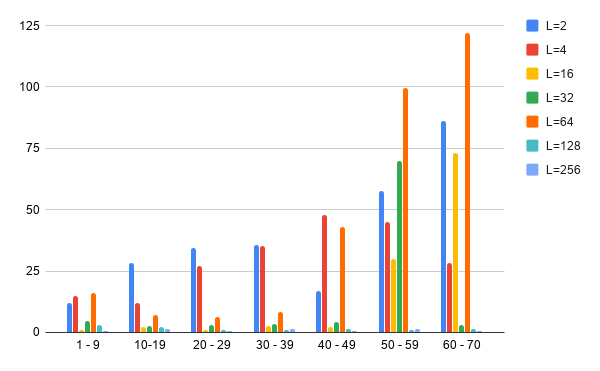
\includegraphics[width = 14 cm]{tests/img/diag_y.png}
    \caption*{Рисунок 12 - Смещение центра по вертикали от числа уровней квантования}
\end{figure}

\begin{table}[h!]
\caption*{Таблица 5 -- Относительное смещение рамки (горизонталь). Кадры 1 - 31 }
\begin{tabular}{|c|c|c|c|c|c|c|c|c|}
\hline
Номер кадра: & L=2 & L=4 & L=8 & L=16 & L=32 & L=64 & L=128 & L=256 \\ \hline
1            & 0.1 & 0.1 & 0.0 & 0.0  & 0.0  & 0.4  & 0.4   & 0.0   \\ \hline
2            & 0.0 & 0.0 & 0.0 & 0.0  & 0.8  & 0.1  & 0.1   & 0.0   \\ \hline
3            & 0.1 & 0.3 & 0.1 & 0.1  & 0.1  & 0.1  & 0.2   & 0.0   \\ \hline
4            & 0.2 & 0.9 & 0.1 & 0.1  & 0.3  & 0.2  & 0.4   & 0.1   \\ \hline
5            & 0.5 & 0.2 & 0.0 & 0.0  & 0.3  & 0.2  & 0.3   & 0.1   \\ \hline
6            & 0.4 & 0.7 & 0.1 & 0.1  & 0.1  & 0.2  & 0.1   & 0.0   \\ \hline
7            & 0.2 & 0.2 & 0.1 & 0.1  & 0.0  & 0.1  & 0.1   & 0.0   \\ \hline
8            & 1.6 & 0.8 & 0.1 & 0.0  & 0.2  & 0.2  & 0.1   & 0.0   \\ \hline
9            & 0.2 & 0.2 & 0.1 & 0.1  & 0.2  & 0.3  & 0.1   & 0.1   \\ \hline
10           & 0.9 & 0.1 & 0.1 & 0.1  & 0.5  & 0.4  & 0.0   & 0.0   \\ \hline
11           & 0.5 & 0.3 & 0.0 & 0.0  & 0.4  & 0.4  & 0.0   & 0.1   \\ \hline
12           & 1.1 & 0.2 & 0.1 & 0.1  & 0.2  & 0.3  & 0.0   & 0.0   \\ \hline
13           & 0.5 & 1.1 & 0.0 & 0.0  & 0.1  & 0.3  & 0.1   & 0.0   \\ \hline
14           & 1.4 & 0.5 & 0.0 & 0.0  & 0.0  & 0.4  & 0.1   & 0.0   \\ \hline
15           & 2.5 & 0.3 & 0.1 & 0.1  & 0.3  & 0.3  & 0.2   & 0.0   \\ \hline
16           & 0.3 & 0.5 & 0.1 & 0.1  & 0.4  & 0.4  & 0.1   & 0.0   \\ \hline
17           & 0.9 & 0.5 & 0.1 & 0.1  & 0.1  & 0.2  & 0.1   & 0.1   \\ \hline
18           & 0.3 & 1.7 & 0.0 & 0.0  & 0.1  & 0.2  & 0.1   & 0.0   \\ \hline
19           & 0.2 & 0.8 & 0.1 & 0.1  & 0.1  & 0.2  & 0.1   & 0.0   \\ \hline
20           & 0.1 & 0.2 & 0.1 & 0.1  & 0.0  & 0.3  & 0.1   & 0.0   \\ \hline
21           & 0.2 & 0.3 & 0.0 & 0.0  & 0.1  & 0.3  & 0.1   & 0.0   \\ \hline
22           & 0.5 & 0.9 & 0.0 & 0.0  & 0.1  & 0.4  & 0.1   & 0.1   \\ \hline
23           & 0.5 & 2.0 & 0.0 & 0.0  & 0.1  & 0.3  & 0.1   & 0.0   \\ \hline
24           & 0.2 & 0.1 & 0.0 & 0.0  & 0.1  & 0.3  & 0.1   & 0.0   \\ \hline
25           & 1.7 & 3.0 & 0.1 & 0.1  & 0.1  & 0.3  & 0.1   & 0.0   \\ \hline
26           & 0.2 & 0.7 & 0.1 & 0.1  & 0.1  & 0.2  & 0.1   & 0.0   \\ \hline
27           & 0.1 & 0.1 & 0.1 & 0.0  & 0.2  & 0.3  & 0.1   & 0.0   \\ \hline
28           & 0.5 & 1.2 & 0.1 & 0.0  & 0.1  & 0.2  & 0.1   & 0.0   \\ \hline
29           & 0.3 & 1.0 & 0.0 & 0.0  & 0.1  & 0.3  & 0.1   & 0.1   \\ \hline
30           & 0.1 & 1.2 & 0.1 & 0.1  & 0.1  & 0.2  & 0.1   & 0.0   \\ \hline
31           & 0.1 & 2.5 & 0.1 & 0.1  & 0.1  & 0.2  & 0.1   & 0.1   \\ \hline
\end{tabular}
\end{table}



\begin{table}[h!]
\caption*{Таблица 6 -- Относительное смещение рамки (горизонталь). Кадры 32 -70 }
\begin{tabular}{|c|c|c|c|c|c|c|c|c|}
\hline
Номер кадра: & L=2 & L=4 & L=8 & L=16 & L=32 & L=64 & L=128 & L=256 \\ \hline
32           & 0.3 & 2.3 & 0.1 & 0.1  & 0.1  & 0.3  & 0.1   & 0.0   \\ \hline
33           & 0.2 & 0.9 & 0.1 & 0.1  & 0.3  & 0.2  & 0.1   & 0.1   \\ \hline
34           & 0.9 & 0.8 & 0.0 & 0.0  & 0.1  & 0.3  & 0.1   & 0.0   \\ \hline
35           & 0.1 & 0.9 & 0.1 & 0.1  & 0.2  & 0.2  & 0.1   & 0.1   \\ \hline
36           & 0.4 & 2.0 & 0.1 & 0.1  & 0.1  & 0.3  & 0.1   & 0.0   \\ \hline
37           & 0.0 & 2.1 & 0.1 & 0.1  & 0.1  & 0.2  & 0.1   & 0.0   \\ \hline
38           & 0.5 & 0.1 & 0.1 & 0.1  & 0.1  & 0.1  & 0.1   & 0.1   \\ \hline
39           & 0.5 & 0.6 & 0.2 & 0.2  & 0.2  & 0.0  & 0.2   & 0.1   \\ \hline
40           & 0.3 & 1.2 & 0.1 & 0.1  & 0.2  & 0.2  & 0.1   & 0.0   \\ \hline
41           & 0.4 & 0.4 & 0.1 & 0.1  & 0.1  & 1.1  & 0.1   & 0.1   \\ \hline
42           & 0.2 & 1.5 & 0.0 & 0.1  & 0.1  & 0.2  & 0.0   & 0.0   \\ \hline
43           & 1.6 & 1.4 & 0.1 & 0.1  & 0.1  & 0.3  & 0.0   & 0.0   \\ \hline
44           & 0.5 & 0.7 & 0.0 & 0.2  & 6.2  & 0.9  & 0.1   & 0.1   \\ \hline
45           & 1.9 & 1.1 & 5.7 & 6.0  & 6.4  & 0.6  & 0.0   & 0.0   \\ \hline
46           & 2.2 & 2.1 & 5.8 & 0.1  & 0.1  & 0.2  & 0.1   & 0.1   \\ \hline
47           & 0.5 & 3.2 & 6.0 & 0.1  & 0.0  & 0.2  & 0.0   & 0.0   \\ \hline
48           & 0.8 & 1.4 & 0.1 & 0.1  & 0.0  & 0.1  & 0.2   & 0.1   \\ \hline
49           & 0.9 & 1.8 & 5.8 & 0.1  & 0.1  & 0.1  & 0.2   & 0.1   \\ \hline
50           & 3.6 & 0.8 & 6.3 & 0.1  & 0.1  & 1.3  & 0.2   & 0.1   \\ \hline
51           & 2.9 & 0.5 & 6.3 & 0.1  & 0.2  & 0.9  & 0.2   & 0.2   \\ \hline
52           & 3.1 & 1.3 & 6.3 & 0.1  & 0.1  & 1.2  & 0.2   & 0.1   \\ \hline
53           & 0.3 & 0.1 & 0.1 & 0.1  & 6.7  & 0.1  & 0.1   & 0.1   \\ \hline
54           & 1.6 & 4.9 & 0.1 & 0.1  & 0.3  & 0.2  & 0.1   & 0.0   \\ \hline
55           & 0.1 & 2.4 & 0.1 & 0.1  & 2.2  & 0.8  & 0.1   & 0.0   \\ \hline
56           & 0.7 & 0.7 & 0.1 & 1.7  & 1.8  & 0.9  & 0.1   & 0.1   \\ \hline
57           & 0.6 & 1.0 & 0.0 & 2.9  & 2.6  & 0.4  & 0.1   & 0.0   \\ \hline
58           & 0.2 & 0.1 & 7.0 & 0.2  & 2.7  & 0.5  & 0.0   & 0.0   \\ \hline
59           & 0.6 & 0.5 & 7.1 & 0.0  & 3.0  & 0.4  & 0.0   & 0.0   \\ \hline
60           & 0.1 & 0.4 & 7.2 & 0.1  & 0.1  & 0.4  & 0.0   & 0.0   \\ \hline
61           & 4.8 & 0.3 & 7.1 & 0.1  & 0.1  & 0.1  & 0.0   & 0.0   \\ \hline
62           & 0.4 & 0.2 & 6.8 & 1.9  & 0.1  & 0.6  & 0.1   & 0.1   \\ \hline
63           & 1.0 & 4.8 & 6.8 & 0.1  & 0.1  & 0.4  & 0.1   & 0.1   \\ \hline
64           & 0.9 & 0.8 & 7.0 & 2.3  & 0.0  & 0.5  & 0.0   & 0.0   \\ \hline
65           & 1.2 & 1.1 & 7.4 & 0.0  & 0.2  & 0.2  & 0.0   & 0.0   \\ \hline
66           & 2.4 & 3.7 & 6.9 & 0.1  & 0.1  & 0.1  & 0.1   & 0.0   \\ \hline
67           & 0.3 & 2.7 & 7.0 & 2.7  & 0.1  & 0.4  & 0.1   & 0.0   \\ \hline
68           & 0.3 & 2.9 & 6.8 & 2.8  & 0.3  & 0.6  & 0.1   & 0.1   \\ \hline
69           & 0.6 & 3.2 & 7.6 & 2.6  & 0.1  & 0.6  & 0.0   & 0.0   \\ \hline
70           & 0.2 & 2.1 & 7.6 & 2.0  & 0.1  & 0.3  & 0.1   & 0.0   \\ \hline
\end{tabular}
\end{table}

\begin{table}[h!]
\caption*{Таблица 7 -- Относительное смещение рамки (вертикаль). Кадры 1 - 31}
\begin{tabular}{|c|c|c|c|c|c|c|c|c|}
\hline
Номер кадра: & L=2  & L=4  & L=8  & L=16 & L=32 & L=64 & L=128 & L=256 \\ \hline
1            & 0.05 & 0.05 & 0.03 & 0.03 & 0.04 & 0.15 & 0.15  & 0.00  \\ \hline
2            & 0.10 & 0.10 & 0.01 & 0.01 & 0.15 & 0.19 & 0.01  & 0.01  \\ \hline
3            & 0.03 & 0.27 & 0.00 & 0.00 & 0.04 & 0.18 & 0.01  & 0.00  \\ \hline
4            & 0.04 & 0.10 & 0.00 & 0.00 & 0.04 & 0.16 & 0.01  & 0.00  \\ \hline
5            & 0.08 & 0.34 & 0.01 & 0.01 & 0.05 & 0.19 & 0.01  & 0.01  \\ \hline
6            & 0.11 & 0.10 & 0.01 & 0.01 & 0.03 & 0.19 & 0.03  & 0.01  \\ \hline
7            & 0.14 & 0.01 & 0.00 & 0.00 & 0.03 & 0.19 & 0.01  & 0.00  \\ \hline
8            & 0.23 & 0.30 & 0.01 & 0.00 & 0.05 & 0.14 & 0.04  & 0.01  \\ \hline
9            & 0.35 & 0.14 & 0.01 & 0.01 & 0.04 & 0.13 & 0.01  & 0.01  \\ \hline
10           & 0.15 & 0.21 & 0.04 & 0.04 & 0.03 & 0.05 & 0.04  & 0.04  \\ \hline
11           & 0.35 & 0.06 & 0.01 & 0.01 & 0.00 & 0.04 & 0.01  & 0.01  \\ \hline
12           & 0.16 & 0.21 & 0.01 & 0.01 & 0.03 & 0.05 & 0.03  & 0.01  \\ \hline
13           & 0.40 & 0.08 & 0.03 & 0.03 & 0.01 & 0.13 & 0.01  & 0.01  \\ \hline
14           & 0.44 & 0.11 & 0.03 & 0.03 & 0.03 & 0.09 & 0.04  & 0.03  \\ \hline
15           & 0.20 & 0.20 & 0.01 & 0.01 & 0.00 & 0.10 & 0.01  & 0.00  \\ \hline
16           & 0.20 & 0.03 & 0.03 & 0.03 & 0.03 & 0.03 & 0.01  & 0.01  \\ \hline
17           & 0.47 & 0.01 & 0.03 & 0.03 & 0.06 & 0.08 & 0.03  & 0.01  \\ \hline
18           & 0.16 & 0.09 & 0.04 & 0.04 & 0.05 & 0.10 & 0.03  & 0.00  \\ \hline
19           & 0.43 & 0.24 & 0.04 & 0.04 & 0.06 & 0.09 & 0.04  & 0.01  \\ \hline
20           & 0.39 & 0.25 & 0.01 & 0.01 & 0.00 & 0.06 & 0.01  & 0.00  \\ \hline
21           & 0.35 & 0.39 & 0.00 & 0.00 & 0.01 & 0.04 & 0.01  & 0.01  \\ \hline
22           & 0.19 & 0.51 & 0.03 & 0.03 & 0.05 & 0.04 & 0.03  & 0.01  \\ \hline
23           & 0.39 & 0.45 & 0.00 & 0.00 & 0.04 & 0.08 & 0.00  & 0.00  \\ \hline
24           & 0.47 & 0.01 & 0.01 & 0.03 & 0.04 & 0.04 & 0.01  & 0.01  \\ \hline
25           & 0.03 & 0.23 & 0.01 & 0.01 & 0.01 & 0.10 & 0.00  & 0.00  \\ \hline
26           & 0.42 & 0.62 & 0.01 & 0.00 & 0.03 & 0.10 & 0.01  & 0.00  \\ \hline
27           & 0.45 & 0.03 & 0.00 & 0.00 & 0.05 & 0.05 & 0.01  & 0.00  \\ \hline
28           & 0.49 & 0.20 & 0.05 & 0.04 & 0.05 & 0.08 & 0.01  & 0.01  \\ \hline
29           & 0.42 & 0.18 & 0.01 & 0.01 & 0.05 & 0.09 & 0.01  & 0.01  \\ \hline
30           & 0.38 & 0.48 & 0.00 & 0.00 & 0.04 & 0.13 & 0.01  & 0.01  \\ \hline
31           & 0.40 & 0.14 & 0.01 & 0.01 & 0.01 & 0.09 & 0.01  & 0.01  \\ \hline
\end{tabular}
\end{table}


\begin{table}[h!]
\caption*{Таблица 8 -- Относительное смещение рамки (вертикаль). Кадры 32 - 70}
\begin{tabular}{|c|c|c|c|c|c|c|c|c|}
\hline
Номер кадра: & L=2  & L=4  & L=8  & L=16 & L=32 & L=64 & L=128 & L=256 \\ \hline
32           & 0.29 & 0.53 & 0.00 & 0.00 & 0.03 & 0.11 & 0.01  & 0.01  \\ \hline
33           & 0.44 & 0.47 & 0.04 & 0.04 & 0.00 & 0.04 & 0.00  & 0.01  \\ \hline
34           & 0.24 & 0.97 & 0.05 & 0.05 & 0.08 & 0.05 & 0.04  & 0.04  \\ \hline
35           & 0.18 & 0.25 & 0.04 & 0.04 & 0.03 & 0.05 & 0.00  & 0.00  \\ \hline
36           & 0.54 & 0.20 & 0.00 & 0.04 & 0.05 & 0.13 & 0.00  & 0.01  \\ \hline
37           & 0.44 & 0.30 & 0.04 & 0.04 & 0.06 & 0.09 & 0.01  & 0.01  \\ \hline
38           & 0.52 & 0.10 & 0.05 & 0.05 & 0.04 & 0.09 & 0.01  & 0.01  \\ \hline
39           & 0.33 & 0.27 & 0.03 & 0.00 & 0.01 & 0.11 & 0.00  & 0.01  \\ \hline
40           & 0.43 & 0.86 & 0.03 & 0.00 & 0.04 & 0.09 & 0.00  & 0.01  \\ \hline
41           & 0.19 & 0.44 & 0.01 & 0.01 & 0.01 & 1.39 & 0.01  & 0.00  \\ \hline
42           & 0.48 & 0.93 & 0.01 & 0.01 & 0.01 & 0.11 & 0.00  & 0.00  \\ \hline
43           & 0.66 & 0.52 & 0.03 & 0.03 & 0.04 & 0.09 & 0.01  & 0.00  \\ \hline
44           & 0.28 & 0.16 & 0.01 & 0.01 & 0.11 & 1.28 & 0.01  & 0.00  \\ \hline
45           & 0.10 & 0.49 & 0.00 & 0.01 & 0.13 & 1.26 & 0.04  & 0.00  \\ \hline
46           & 0.40 & 0.53 & 0.06 & 0.03 & 0.03 & 0.09 & 0.01  & 0.00  \\ \hline
47           & 0.18 & 0.13 & 0.06 & 0.05 & 0.03 & 0.09 & 0.01  & 0.01  \\ \hline
48           & 0.30 & 0.29 & 0.05 & 0.05 & 0.04 & 0.08 & 0.03  & 0.01  \\ \hline
49           & 0.34 & 0.66 & 0.08 & 0.04 & 0.04 & 0.06 & 0.04  & 0.03  \\ \hline
50           & 0.35 & 0.47 & 0.11 & 0.06 & 0.06 & 1.24 & 0.01  & 0.00  \\ \hline
51           & 0.18 & 0.43 & 0.08 & 0.08 & 0.03 & 1.25 & 0.04  & 0.05  \\ \hline
52           & 0.09 & 0.06 & 0.03 & 0.04 & 0.03 & 1.26 & 0.03  & 0.03  \\ \hline
53           & 0.56 & 0.88 & 0.05 & 0.03 & 0.08 & 0.08 & 0.01  & 0.01  \\ \hline
54           & 0.59 & 0.00 & 0.04 & 0.03 & 0.01 & 0.09 & 0.00  & 0.00  \\ \hline
55           & 0.61 & 0.21 & 0.04 & 0.03 & 1.40 & 1.31 & 0.01  & 0.01  \\ \hline
56           & 1.50 & 0.48 & 0.03 & 1.41 & 1.43 & 1.31 & 0.00  & 0.03  \\ \hline
57           & 0.19 & 0.73 & 0.03 & 1.43 & 1.40 & 1.33 & 0.01  & 0.01  \\ \hline
58           & 0.44 & 0.47 & 0.28 & 0.03 & 1.44 & 1.34 & 0.01  & 0.00  \\ \hline
59           & 1.57 & 1.00 & 0.27 & 0.03 & 1.47 & 1.28 & 0.00  & 0.01  \\ \hline
60           & 1.52 & 0.37 & 0.27 & 0.01 & 0.01 & 1.29 & 0.03  & 0.00  \\ \hline
61           & 0.09 & 0.56 & 0.25 & 0.03 & 0.01 & 1.28 & 0.01  & 0.00  \\ \hline
62           & 0.15 & 0.21 & 0.28 & 1.44 & 0.03 & 1.28 & 0.01  & 0.00  \\ \hline
63           & 1.65 & 0.09 & 0.33 & 0.05 & 0.04 & 1.28 & 0.00  & 0.01  \\ \hline
64           & 0.52 & 0.09 & 0.33 & 1.36 & 0.00 & 1.24 & 0.01  & 0.00  \\ \hline
65           & 1.49 & 0.19 & 0.35 & 0.00 & 0.01 & 1.26 & 0.01  & 0.00  \\ \hline
66           & 0.20 & 0.03 & 0.35 & 0.03 & 0.03 & 1.29 & 0.04  & 0.03  \\ \hline
67           & 1.67 & 0.56 & 0.39 & 1.35 & 0.08 & 1.31 & 0.01  & 0.00  \\ \hline
68           & 1.63 & 0.27 & 0.40 & 1.41 & 0.09 & 1.29 & 0.01  & 0.00  \\ \hline
69           & 0.63 & 0.04 & 0.32 & 1.39 & 0.03 & 1.29 & 0.01  & 0.01  \\ \hline
70           & 0.40 & 0.90 & 0.37 & 1.40 & 0.01 & 1.33 & 0.01  & 0.01  \\ \hline
\end{tabular}
\end{table}

\begin{figure}[h!]
    \centering
    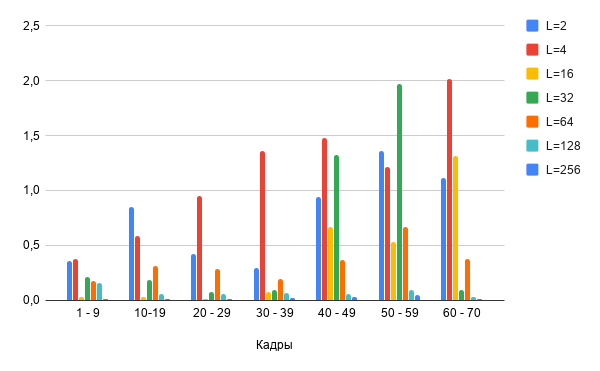
\includegraphics[width = 14 cm]{tests/img/diag_rlt_disp_x.png}
    \caption*{Рисунок 13 - Относительное смещение (горизонталь) от уровней квантования}
    \label{fig:my_label}
\end{figure}

\begin{figure}[h!]
    \centering
    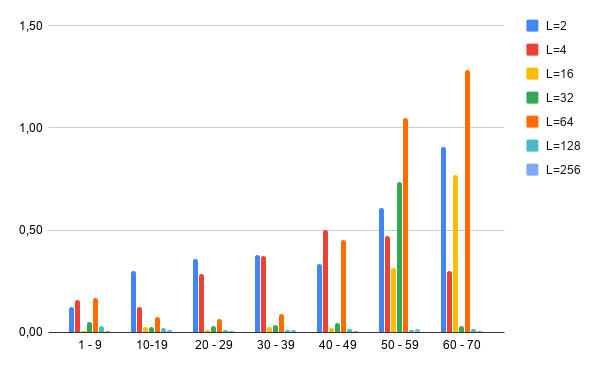
\includegraphics[width = 14 cm]{tests/img/diag_rlt_disp_y.png}
    \caption*{Рисунок 14 - Относительное смещение (по вертикали) от уровней квантования}
    \label{fig:my_label}
\end{figure}
\end{document}